\subsection{Herramientas utilizadas}

Para la implemetaci\'on del analizador l\'exico y sint\'actico de la gram\'atica propuesta, se decidi\'o utilizar las herramientas propuestas por la c\'atedra. Las mismas son:

\begin{itemize}

\item[•] \textbf{PLY}: \href{http://www.dabeaz.com/ply/}{Python Lex Yacc} es una implementaci\'on de las herramientas \textbf{Lex} \textbf{Yacc}
%\href{http://www.wikibooks.org}{Lex} y \href{http://www.wikibooks.org}{Yacc} en pyhton.

\item[•] \textbf{VPython}: \href{http://vpython.org/index.html}{Visual Python} es una herramienta para programaci\'on gr\'afica.

\end{itemize}

\subsection{Decisiones para la implementaci\'on}

Para los tokens, la decisión tomada para este entrega es la explicada conjuntamente entre los items \textbf{Cambios para la reentrega} y \textbf{Descripción de la gramática}
\\
\\
Luego, para poder implementar comentarios, y que se pueda ignorar el contenido, se utiliz\'o la notaci\'on de \textbf{t\_ignore} seguido de un nombre declarativo para lo que se desee ignorar, por ej\'emplo en este caso, \textbf{t\_ignore\_comment}.
La definición de su expresión regular correspondiente permite tener comillas dentro del comentario, siempre y cuando estas comillas esten escapadas con un $\backslash$
\\
\\
En el caso de analizador sint\'actico se decidi\'o utilizar un diccionario para guardar las transformaciones de un elemento.
\\
\\
Una vez que se tiene una expresi\'on v\'alida, es decir que pas\'o por el analizador l\'exico, y luego, el sint\'actico, y no produjo error, se desea visualizar dicha expresi\'on, ya que la misma describe un objeto 3D. Para este paso de la visualizaci\'on, se aprovech\'o la herramienta visual python, junto con una jerarqu\'ia de clases que m\'as adelante se describe, que la misma va a representar un comportamiento para l correcta visualizaci\'on de dicho objeto, esto se debe a que en ciertas expresiones que contienen la disyunci\'on de objetos 3D, para la visualizaci\'on del objeto total, a cada objeto dentro de la disyunci\'on le corresponde una probabilidad de ser visualizado. Este comportamiento se engloba en una clase descripta posteriormente.
%~ 
%~ Al momento de poder decir que una expresi\'on es v\'alida, es decir, que pudo pasar por el analizador l\'exico, luego por el sint\'actico y no produjo error, debemos poder ejecutarla correctamente. Para esto se tuvo que tomar otra decisi\'on, ya que la utilizaci\'on de la herramienta visual python por si sola no alcanzaba para los objetivos de este trabajo pr\'actico. Esto se debe a que al momento de mostrar esta expresi\'on, queremos contemplar ciertas probabilidades y relaciones con el \textbf{ \& } o el \textbf{ \textbar } que la herramienta por si sola no contempla. 
%~ Para ello, se implemento una jerarqu\'ia de clases para poder mostrar acorde a los requerimientos de este trabajo pr\'actico.


\subsection{C\'odigo}

El c\'odigo se dividi\'o en 6 achivos:
\begin{itemize}
\item[•] \textbf{lexer.py:} Este archivo contiene la implementaci\'on del analizador l\'exico. Para dicha implementaci\'on se defini\'o la lista de tokens, presentada en la secci\'on de descripci\'on de la gram\'atica, y luego las expresiones regulares para cada token, incluyendo las expresiones de lo que se desea ignorar, como por ejemplo los comentarios. Luego, la llamada a la herramienta a \textbf{lex.lex()} para generar el analizador l\'exico de la gram\'atica propuesta.

\item[•] \textbf{yacc.py:} En este archivo se encuentra la implementaci\'on del analizador sint\'actico, que incluye las definiciones de las producciones definidas en la secci\'on de descripci\'on de la gram\'atica. Seg\'un a qu\'e expresi\'on corresponde se define lo que se desea guardar en el diccionario. Por \'ultmo, la llamada a la herramienta \textbf{yacc.yacc()} para generar el analizador sint\'actico. Cabe destacar que para generar el analizador sint\'actico se requiere de la lista de tokens y de analizador l\'exico, por lo que ambos se incluyen del archivo anterior.

\item[•] \textbf{definition.py:} Este archivo contiene la implementaci\'on de los procedimientos requeridos para la visualizaci\'on de los resultados, el mismo se implement\'o en una jerarqu\'ia de clases para realizar la visualizaci\'on de los objetosacorde a las probabilidades deseadas, junto con las diferentes formas de visualizar. La clase padre es \textbf{Definition} que contiene una funci\'on para cada forma posible de mostrar objetos. 

\item[•] \textbf{transformation.py} Este archivo contiene la definici\'on de la clase Transformation, que representa el conjunto la matriz asociada a la representaci\'on espacial, el arreglo que representa los canales de color (RGB) y la profundidad m\'axima.

\item[•] \textbf{dictionaries.py} Este archivo contiene funciones que asocian los elementos primitivos a las representaci\'ones correspondientes definidas como subclases de la clase definitions y funciones que asocian un string a su transformaci\'on.

\item[•] \textbf{functions.py} Este archivo contiene funciones auxiliares.
\end{itemize}

A continuaci\'on se presenta el c\'odigo contenido en cada archivo.

\newpage
\subsubsection{lexer.py}

\lstinputlisting[language=Python,breaklines=true]{../lexer.py}

%revisar nombres de funciones 
En el c\'odigo previamente mostrado se puede ver la lista de tokens utilizados, luego la expresi\'on regular para cada uno. Se pueden observar, que adem\'as hay unas funciones auxiliares, tales como \textbf{isPrimitive} e \textbf{isTransformation}, que fueron implementadas para el cambio de la expresi\'on regular de \textbf{RULE\_NAME}. Las mismas lo que hacen es verificar si un string est\'a contenido en la lista de keywords (tanto si es un elementos primitivo o una transformacion), que se corresponden a los antiormente presentados como tokens.

\newpage
\subsubsection{yacc.py}

\lstinputlisting[language=Python,breaklines=true]{../yacc.py}

En el archivo Python presentado anteriormente se puede observar la implementaci\'on de las reglas sem\'anticas, con el cambio en las reglas de rotaci\'on, 

\newpage
\subsubsection{definition.py}

\lstinputlisting[language=Python,breaklines=true]{../definition.py}

En el c\'odigo presentado anteriormente se muestran una sucesi\'on de clases implementadas para la visualizaci\'on de las cadenas aceptadas por este lenguaje. Principalmente para tener una representaci\'on arborea del armado de cada definici\'on.

A continuaci\'on se describe brevemente cada clase y porqu\'e se decidi\'o generar la misma.

\begin{itemize}

\item \textbf{Class Definition:} La misma es una clase abstracta que define un comportamiento gen\'erico y sus subclases 
definir\'an comportamientos m\'as espec\'ificos seg\'un corresponda, si cada subclase tiene una transformaci\'on asociada y se le puede aplicar transformaci\'on.

\item \textbf{Class ANDDefinition:}Esta clase representa una lista de conjunciones de definiciones, cuando se desean mostrar estas definiciones, el comportaminto esperado es que se muestre cada una de las definiciones de dicha lista.

\item \textbf{Class ORDefinition:} Similar al caso anterior, esta clase representa una lista de disyunciones de definiciones y al querer mostrar dicha lista el comportamiento deseado es que se elija aleatoriamente un elemento de la lista y se muestre dicha definici\'on.

\item \textbf{Class POWDefinition:}Esto representa el caso de una definici\'on elevada a la N, el comportamiento esperado al mostrar esta definici\'on va a depeder de la definici\'on sobre la que habla, ya que va a ser una instancia de alguna de las clases anteriores y acorde a cual sea se definir\'a su comportamiento.

\item \textbf{Class CorcheteDefinition:} Esta clase representa una definici\'on entre corchetes, por lo que al igual que la clase descripta anteriormente va a definir el comportamiento la instancia de la definici\'on que est\'a contenida entre los corchetes.

\item \textbf{Class RULEDefinition:} La misma representa cuando una definici\'on hace referencia a un nombre de regla definida. 

\item \textbf{Class LessGRaterDefinition:} Esta clase representa a una definici\'on entre $<>$

\item \textbf{Class VOID:} Representa el elemento primitivo \_

\item \textbf{Class BALL:} Representa el elemento primitivo ball.

\item \textbf{Class BOX:}  Representa el elemento primitivo box.
%AGREGAR EJEMPLOS DE INPUT y como es el arbol uno chiquito y ademas uno de corchete y pow

\end{itemize}

Para una mejor comprensi\'on de lo anteriormente dicho, se puede observar el siguiente ej\'emplo:

\lstinputlisting[language=Python,breaklines=true]{../Ejemplos/eg09b.peg}

\centerline{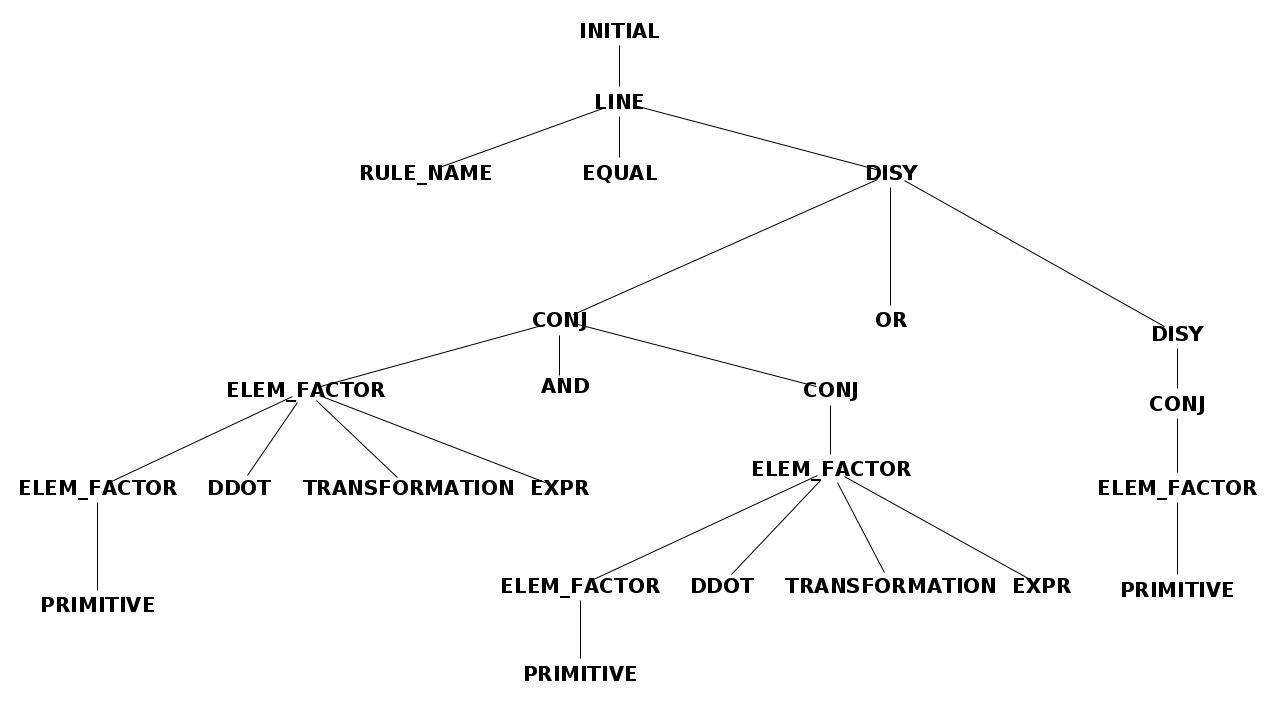
\includegraphics[scale=0.40]{arboles_derivacion/Ejemplo_and_or1.jpg}}

Este ejemplo debe mostrar, o bien, la parte del AND  (que la misma debe mostrar juntos los dos objetos del AND), o bien, el VOID.

De esta forma se va a obtener la clase padre que va a ser una instancia de ORDefinition y luego, el ANDDefinition, generando en conjunto el comportamiento deseado.
\\
\\
El siguiente ejemplo muestra otro caso, con otros operadores:

\lstinputlisting[language=Python,breaklines=true]{../Ejemplos/eg14.peg}

\centerline{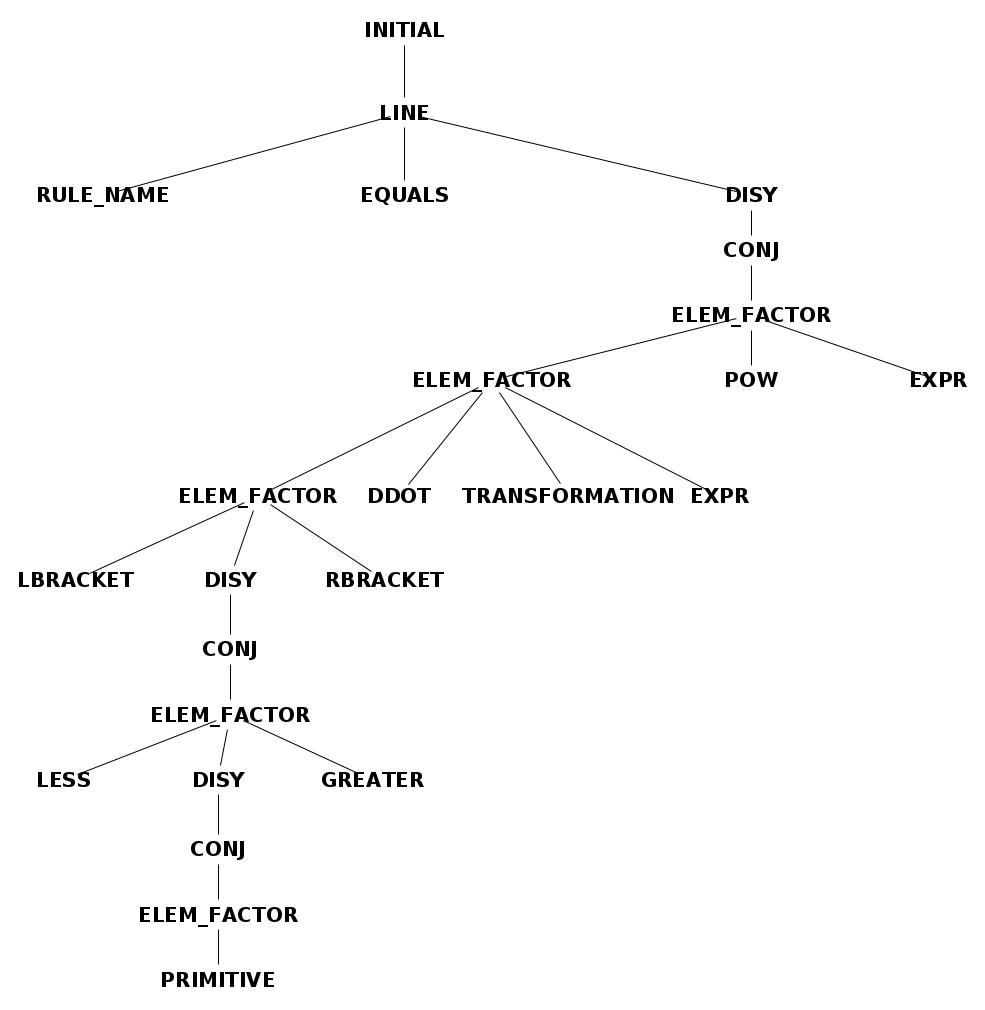
\includegraphics[scale=0.40]{arboles_derivacion/brackets_less_greater1.jpg}}

En este ejemplo se tiene una combinaci\'on de varios operadores de la visualizaci\'on, por un lado, la potenciaci\'on que genera una repetici\'on del elemento al que se le aplica la misma. Por otro lado, los operadores $< >$ que describen un comportamiento opcional en cuanto a la visualizaci\'on, y, por \'ultimo, la agrupación, dada por los $[ ]$ que agrupar\'a, en este caso el efecto de la potenciaci\'on. \\
En este ejemplo se puede observar que respecto a las clases previamente descriptas, se va a tener una jerarqu\'ia de las mismas generando el comportamiento esperado para este ejemplo.\\
\\

\newpage
\subsubsection{transformation.py}

\lstinputlisting[language=Python,breaklines=true]{../transformation.py}

El c\'odigo recientemente presentado muestra la clase Transformation, que como se dijo anteriormente representa en conjunto la matriz de representaci\'on espacial,vector de canales de colores rgb, y la profundidad maxima.
A una instancia de esta clase se le puede aplicar una transformaci\'on con otra instancia de la misma clase. El resultado de dicha operaci\'on es la siguiente:
Supongamos 2 instancias t1 y t2, y la operaci\'on es t1.transform(t2)
\begin{itemize}
\item[•] La matriz de representaci\'on espacial resultante es premultiplicar la matriz de t1 por la matriz de t2. 
\item[•] Con respecto al vector de colores, es el producto interno de ambos vectores.
\item[•] La profundidad m\'axima resultante es la minima entre la de t1 y t2. 
\end{itemize}

\newpage
\subsubsection{dictionaries.py}

\lstinputlisting[language=Python,breaklines=true]{../dictionaries.py}
\newpage
\subsubsection{functions.py}

\lstinputlisting[language=Python,breaklines=true]{../functions.py}

\newpage
\subsubsection{Modo de uso}
El programa se utiliza por medio de una consola de comandos, de la siguiente manera:\\
\textbf{ python grapher.py pathArchivo} \\ 
Donde \'pathArchivo\' se cambia por el archivo a ejecutar.
\\
Por ejemplo:\\
\\
\texttt{python grapher.py ejemplo\_cube.peg}
\\
\\
donde el archivo ejemplo\_cube.peg, contiene el programa a compilar y correr.
